\chapter{Introducción}
\title{Introducción}
\label{cap:Introduccion}

\section{Astronomía}
La astronomía es la ciencia que se ocupa del estudio de los cuerpos celestes del universo, los planetas y sus satélites, los cometas y meteoroides, las estrellas y la materia interestelar, los sistemas de materia oscura, estrellas, gas y polvo llamados galaxias y los cúmulos de galaxias, así como sus movimientos, los fenómenos ligados a ellos y las leyes que los rigen. \\

La palabra, como tal, proviene del latín astronomía. La astronomía ha formado parte de la historia de la humanidad considerándola como la ciencia más antigua. Civilizaciones como la azteca, la maya y la inca, así como la egipcia, la china y la griega alcanzaron un grado tal de conocimientos que son tenidos por fundamentales para la posterior evolución de esta disciplina, considerándola como esencial para otras ciencias como la matemática o la física.\\

Su registro y la investigación de su origen se produce a partir de la información que llega de ellos a través de la radiación electromagnética o de cualquier otro medio.\\

Es una de las pocas ciencias en las que los \textit{amateurs} también pueden desempeñar un papel activo, especialmente en el descubrimiento y seguimiento de fenómenos como curvas de luz de estrellas variables, descubrimiento de asteroides y cometas, etc.\\

En sus inicios, la astronomía tenía una aplicación práctica para conocer los ciclos de los astros y establecer medidas de tiempo que permitieran determinar, entre otras cosas, el momento propicio para la siembra y la cosecha. En los pueblos antiguos, los astros se consideraban como divinidades y el estudio de sus posiciones resultaba esencial para determinar sus influencias sobre los acontecimientos terrenales. Por este conjunto de razones la astronomía fue, en todas las civilizaciones del pasado, una ciencia tanto al servicio del poder civil como del religioso.\\

Antiguamente se ocupaba, únicamente, de la observación y predicciones de los movimientos de los objetos visibles a simple vista, quedando separada durante mucho tiempo de la Física. En Sajonia-Anhalt, Alemania, se encuentra el famoso Disco celeste de Nebra, que es la representación más antigua conocida de la bóveda celeste. Quizá fueron los astrónomos chinos quienes dividieron, por primera vez, el cielo en constelaciones. Los antiguos griegos hicieron importantes contribuciones a la astronomía, entre ellas, la definición de magnitud. La astronomía precolombina poseía calendarios muy exactos y parece ser que las pirámides de Egipto fueron construidas sobre patrones astronómicos muy precisos.\\

Fue probablemente Eratóstenes quien diseñara la esfera armilar que es un astrolabio para mostrar el movimiento aparente de las estrellas alrededor de la tierra.\\

La astronomía observacional estuvo casi totalmente estancada en Europa durante la Edad Media, a excepción de algunas aportaciones como la de Alfonso X el Sabio con sus tablas alfonsíes, o los tratados de Alcabitius, pero floreció en el mundo con el Imperio persa y la cultura árabe. Al final del siglo X, un gran observatorio fue construido cerca de Teherán (Irán), por el astrónomo persa Al-Khujandi, quien observó una serie de pasos meridianos del Sol, lo que le permitió calcular la oblicuidad de la eclíptica. También en Persia, Omar Khayyam elaboró la reforma del calendario que es más preciso que el calendario juliano acercándose al Calendario Gregoriano.\\

Durante siglos, la visión geocéntrica de que el Sol y otros planetas giraban alrededor de la Tierra no se cuestionó. En el Renacimiento, Nicolás Copérnico propuso el modelo heliocéntrico del Sistema Solar. Su trabajo De Revolutionibus Orbium Coelestium fue defendido, divulgado y corregido por Galileo Galilei y Johannes Kepler, autor de Harmonices Mundi, en el cual se desarrolla por primera vez la tercera ley del movimiento planetario.\\

Galileo añadió la novedad del uso del telescopio para mejorar sus observaciones. La disponibilidad de datos observacionales precisos llevó a indagar en teorías que explicasen el comportamiento observado. Al principio sólo se obtuvieron reglas como las leyes del movimiento planetario de Kepler, descubiertas a principios del siglo XVII.\\

Fue Isaac Newton quien extendió hacia los cuerpos celestes las teorías de la gravedad terrestre y conformando la Ley de la gravitación universal, inventando así la mecánica celeste, con lo que explicó el movimiento de los planetas y consiguiendo unir el vacío entre las leyes de Kepler y la dinámica de Galileo. Esto también supuso la primera unificación de la astronomía y la física.\\

Tras la publicación de los Principios Matemáticos de Isaac Newton (que también desarrolló el telescopio reflector), se transformó la navegación marítima. A partir de 1670, utilizando instrumentos modernos de latitud y los mejores relojes disponibles se ubicó cada lugar de la Tierra en un planisferio o mapa, calculando para ello su latitud y su longitud. Los requerimientos de la navegación supusieron un empuje para el desarrollo progresivo de observaciones astronómicas e instrumentos más precisos, constituyendo una base de datos creciente para los científicos.\\

A finales del siglo XIX se descubrió que, al descomponer la luz del Sol, se podían observar multitud de líneas de espectro , regiones en las que había poca o ninguna luz. \\

Se descubrió que las estrellas eran objetos muy lejanos y con el espectroscopio se demostró que eran similares al Sol, pero con una amplia gama de temperaturas, masas y tamaños. La existencia de la Vía Láctea como un grupo separado de estrellas no se demostró hasta el siglo XX, junto con la existencia de galaxias externas y, poco después, la expansión del universo, observada en el efecto del corrimiento al rojo. La astronomía moderna también ha descubierto una variedad de objetos exóticos como los quásares, púlsares, radiogalaxias, agujeros negros, estrellas de neutrones, y ha utilizado estas observaciones para desarrollar teorías físicas que describen estos objetos. \\

Durante el siglo XX, la espectrometría avanzó, en particular, como resultado del nacimiento de la física cuántica, necesaria para comprender las observaciones astronómicas y experimentales.\\

La astronomía moderna se divide en varias ramas: astrometría, el estudio mediante la observación de las posiciones y los movimientos de estos cuerpos; mecánica celeste, el estudio matemático de sus movimientos explicados por la teoría de la gravedad; astrofísica, el estudio de su composición química y su condición física mediante el análisis espectral y las leyes de la física, y cosmología, el estudio del Universo como un todo.\\

\section{Observatorio e Instrumental Astronómico}
La denominación y el edificio conocido como Observatorio Astronómico, lugar desde donde se estudian y controlan los cambios, los movimientos y las leyes que  rigen los astros, ha sufrido grande cambios con el paso del tiempo. En la antigüedad, dado que la astronomía estaba ligada a la religión y por tanto a los templos, estos eran los lugares que servían para hacer de ellos observatorios astronómicos. \\

Fue ya en la Edad Media cuando el observatorio comenzó a ser un lugar en el cual se reunían los astrónomos y en él se fueron disponiendo los diferentes instrumentos o herramientas que facilitaban el estudio de aquellas personas, profesionales o \textit{amateurs}, que se dedicaban a esta disciplina.
Después de las primeras décadas del siglo XX, los astrónomos se veían en la obligación de alejarse de la ciudad debido a la contaminación lumínica y química que en ella se produce. Es en este momento histórico cuando comenzaron a construirse los observatorios astronómicos, siguiendo en la actualidad ubicándose en lugares desérticos y elevados para conseguir trabajar con un cielo oscuro, libre de contaminación lumínica y consiguiendo que el número de días serenos sea más elevado.\\

Por otra parte, se denomina instrumental astronómico al conjunto de instrumentos a disposición del astrónomo para complementar y facilitar sus observaciones.
A continuación, se pasa a describir parte del instrumental más importante que podemos encontrar en un observatorio.\\


\subsection{Telescopio}
El telescopio es un instrumento cuya función principal es recoger la luz de un objeto lejano y ampliarlo. Está considerado como el artífice de la astronomía moderna. \\
\begin{figure}[htb]
\centering
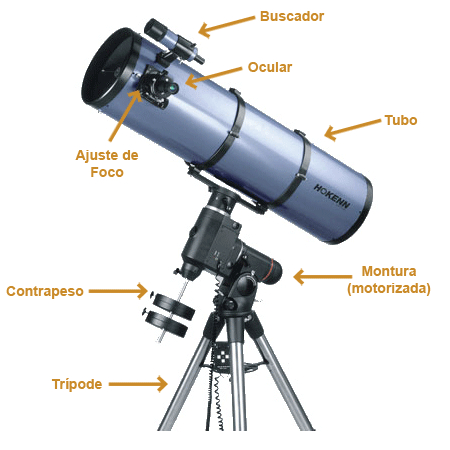
\includegraphics[width=0.6\textwidth]{./imagenes/telescopio}
\caption{Telescopio Astronómico (http://blog.astroaficion.com/)} \label{fig:telescopio}
\end{figure}

\subsection{Cámara CCD}
\subsection{Montura}
\subsection{Enfocador}
\subsection{Rueda Portafiltros}
\subsection{Cúpula}
\subsection{Óptica Adaptativa}
\subsection{Estación Meteorológica}
\subsection{Controlador de Dispositivos}
